\section{An Overview of BIP32-based HD Wallets}
\label{sec:bip32}

Hierarchical Deterministic Wallets (HD wallets, for short) in the cryptocurrency
domain derive from the BIP32 specification%
\footnote{\url{https://github.com/bitcoin/bips/blob/master/bip-0032.mediawiki}.
  Last access, December 13th, 2021.}
The motivation behind creating this type of wallets is clear if one thinks about
how typical cryptocurrency systems work: each address is associated with a key
pair and, in order to achieve high security and privacy levels, it is best to
limit the reusage of addresses (thus, key pairs). Therefore, a too high number
of needed key pairs is quickly reached. If each key is generated independently
at random, management becomes too complex -- especially, if several devices
are expected to be synchronised. As a solution to this challenge, a hierachical
tree-based data structure was proposed, in which each parent node can be used to
derive multiple child nodes, deterministically. This approach seems also useful
to foster some sort of separation -- i.e., create sub-trees that are
(computationally) independent from one another, in the sense that a compromise
in one does not lead to a compromise in the other. Typically, the root node
of the tree is derived from a seed encoded as a mnemonic. BIP39%
\footnote{\url{https://github.com/bitcoin/bips/blob/master/bip-0039.mediawiki}.
  Last access, December 13th, 2021.} is the main specification for this purpose.

In this section, we give a brief overview of the BIP32 specification, and
provide a ``full path'' from mnemonic to key pair. To avoid repeating already
well documented processes, the overview will refer to the specifications when
appropriate.
%
In a final subsection, we will also overview how does all this apply to the
Cardano Lightwallet and Atala Prism cases.

\subsection{Main Specifications}

While the main specification is BIP32, it essentially gives the basic guidelines
to create HD wallets. To avoid ambiguity leading to incompatible
implementations, BIP43%
\footnote{\url{https://github.com/bitcoin/bips/blob/master/bip-0043.mediawiki}.
  Last access, December 13th, 2021.} and BIP44%
\footnote{\url{https://github.com/bitcoin/bips/blob/master/bip-0044.mediawiki}.
  Last access, December 13th, 2021.} specify how to organize HD wallets so
that the resulting tree structure enables the most common use cases (which, at
least initially, focus on the cryptocurrency scenario). In addition, the
specification that defines how to encode (pseudo-)random bitstrings as
mnemonic is given in BIP39.

\subsection{Main Concepts}

\begin{description}
\item[HD wallet tree structure.] HD wallets are organised as trees, where the
  root node is directly derived from the main seed (typically, a mnemonic-encoded
  random string). We denote the root level with level $0$, and all descendants
  with increasing numbers. A level other than the root level can have an
  arbitrary number of nodes.
\item[(Child) Index.] The child index just identifies how many childs can be (or
  have been) created before the current child, at the current depth of the tree.
  We assume $0$ to be the first index.
\item[Chaincode.] To introduce extra ``non-determinism'' in the way child keys
  are derived from parent keys, part of the pseudo-randomly derived data is
  used as key for pseudo-random derivations of lower levels. This part of the
  derived data is referred to as chaincode. We will denote the chaincode of the
  $j$-th node at level $i$ of the tree with $c_{i,j}$. This data should be kept
  secret; otherwise, entire subtrees can be compromised.
\item[Extended keys.] An extended public (resp. private) key is composed by the
  public (resp. private) key and the chaincode.  
\item[Hardened child keys.] A hardened child key can only be derived from the
  parent private key, and the parent key chaincode. 
\item[Non-hardened child keys.] A non-hardened child key can be derived both
  from the parent private and parent public key, and the parent key chaincode.
\end{description}

\paragraph{Hardened vs non-hardened child derivation.} Basically, child nodes
are derived as rerandomizations of their parent node private key. The
pseudo-random data used for rerandomization can be derived from the parent
private extended key, or from the parent public extended key. The former case is
referred to as hardened derivation, and the latter as non-hardened derivation.
In a nutshell, this means that hardened child keys (private or public) can only
be derived from their parent private key, but not from their parent public key.
Naturally, child private keys can only be derived from parent private keys.

For self-containedness, \figref{fig:childderivation} shows the different
algorithms to derive child keys from a parent keys, excluding some details. For
the full algorithms, we refer to BIP32.

\begin{figure}[ht!]
  \begin{minipage}[t]{0.55\textwidth}
    \procedure{$prv2HardChild$ \pccomment{Parent private key $\rightarrow$ $i$-th Child hardened key pair}}{
      \pcind I \gets HMAC(c_{par}, k_{par}, i) \\
      \pcind k^h \gets (k_{par} + Left(I)) \bmod n; K^h \gets k^hG; c^h \gets Right(I) \\
      \pcind \pcreturn (k^h,K^h,c^h) \\
    }
    \procedure{$prv2NonHardChild$ \pccomment{Parent private key $\rightarrow$ $i$-th Child non-hardened key pair}}{    
      \pcind I \gets HMAC(c_{par}, K_{par}, i) \\
      \pcind k^{nh} \gets (k_{par} + Left(I)) \bmod n; K^{nh} \gets k^{nh}G; c^{nh} \gets Right(I) \\
      \pcind \pcreturn (k^{nh},K^{nh},c^{nh}) \\      
    }
    \procedure{$pub2NonhardPubChild$ \pccomment{Parent public key $\rightarrow$ $i$-th Child non-hardened public key}}{      
      \pcind I \gets HMAC(c_{par}, K_{par}, i) \\
      \pcind K^{nh} \gets Left(I)G + K_{par}; c^{nh} \gets Right(I) \\
      \pcind \pcreturn (K^{nh},c^{nh}) 
    }    
  \end{minipage}
  \caption{Algorithms for child derivation. $k_{par},K_{par},c_{par}$ denote the
    parent's public key, private key, and chaincode, respectively. $k,K,c$
    denote the resulting child's private key, public key, and chaincode. $h$ or
    $nh$ superscripts denote hardened or non-hardened derivation. $Left$
    (resp. $Right$) divides a bitstring in two equal parts, and takes the left
    (resp. right) half. The result of both $Left$ and $Right$ can be interpreted
    as a scalar, and thus multipled by points in the elliptic curve, such as $G$,
    which is the base point, or public keys, which also are points in the
    curve.}
  \label{fig:childderivation}
\end{figure}

\paragraph{Isolation of HD wallet subtrees.} In the following section, we use
the concept of isolated and non-isolated subtrees. This is something that is
only indirectly mentioned in the BIPs and other related works, but which is of
crucial importance in order to limit the impact of compromised keys. Namely,
assume that a child key is derived in non-hardened mode. Then, if the extended
parent public key is leaked, as well as the private (non-extended) non-hardened
child key, it is possible to extract the parent private key -- and, therefore,
all the keys (private and public; hardened or not) that derive from it. If child
keys are derived in hardened mode, this does not apply. For the sake of clarity,
we illustrate the difference through the diagram in \figref{fig:isolation}.

\begin{figure}[ht!]
  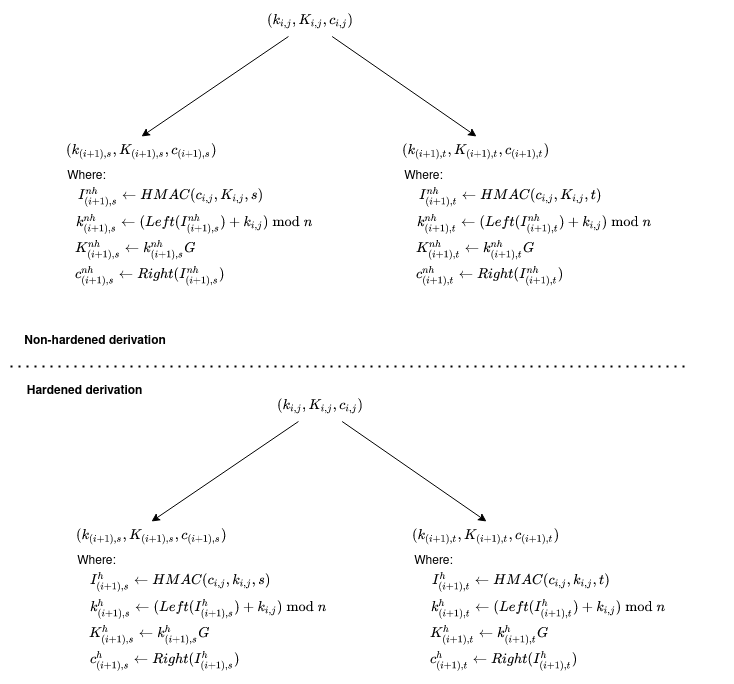
\includegraphics[width=\textwidth]{figures/child_derivation.png}
  \caption{Sub-tree isolation through hardened child derivation. $G$ is the
    base point of the underlying elliptic curve, and $n$ is the order of
    the associated group.}
  \label{fig:isolation}
\end{figure}

For instance, assume that the extended public key $(K_{i,j}, c_{i,j})$ is
compromised, along with its child private non-hardened key $k^{nh}_{(i+1),t}$.
Then, it is straightforward  to recompute the \emph{parent} private key
$k_{i,j}$ (independently on whether it was derived in hardened mode or not) as:
$k_{i,j} \leftarrow (K_{(i+1),t}^{nh} - Left(I_{(i+1),t}^{nh})) \bmod n$.
Obviously, given the parent private key $k_{i,j}$, it is straightforward to
derive all its descendants (hardened or not), as well as possibly and
recursively apply the same strategy, if the just recovered parent key was
derived in non-hardened mode.

\subsection{From Mnemonic to Key Pairs: High-level Overview}

The following description is based on BIP39 for the processing of mnemonics,
and BIP44 (which is a restriction of BIP43 and BIP32) for general structure of
an HD wallet, which we depict in \figref{fig:bip44-tree}.

\begin{figure}[ht!]
  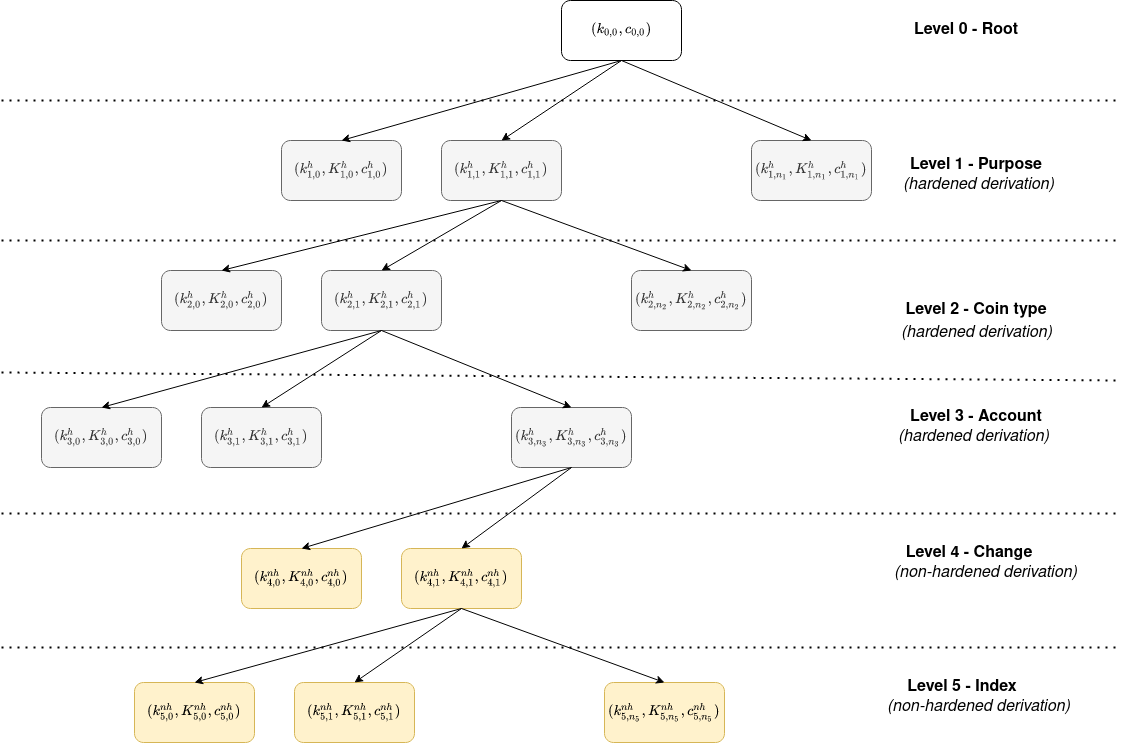
\includegraphics[width=\textwidth]{figures/bip44_tree.png}
  \caption{Basic tree structure of a BIP44-based HD wallet.}
  \label{fig:bip44-tree}
\end{figure}

\paragraph{From (pseudo-)random bitstrings to mnemonics, and back.} %
Mnemonics encode randomness in human-readable form. BIP39 is the main
specification for this. Roughly, between 128 and 256 random bits (in multiples
of 32) are generated, a checksum (the first few bits of a hash of these random
bits) is concatenated, and the result is divided in chunks of 11 bits. Each of
these chunks is used as index to a predefined dictionary of words. The result
is a mnemonic of 12 to 24 words. To convert from mnemonic to random bits, just
the inverse process has to be followed (verifying the checksum).

Given the mnemonic, it is converted back into a bitstring as just described.
Then, this bitstring is processed with an HMAC function, using the string
``Bitcoin seed'' as key \needcite~based on SHA512 -- hence producing 512 bits of
output. The first 256 bits are set as master secret key, and the last 256 bits
as master chaincode (i.e., $k_{0,0}$ and $c_{0,0}$, in our previous notation).

\paragraph{Layer 1: \emph{isolated} subtrees per \texttt{purpose}} %
The first layer of a BIP44-compatible HD wallet is composed of up to $2^{31}$
nodes of hardened childs: i.e., layer 1 is composed of childs $(1,2^{31})$
to $(1,2^{62}-1)$, where the second element in the pair is the $i$ value used
in the child derivation processes, and denotes for what ``purpose'' the
descendant keys will be used -- this roughly translates to the system (e.g.,
Bitcoin, Cardano... or even non-blockchain systems, in theory).

Note that, being layer 1 computed in hardened mode, a private key compromise
of one node in layer 1 does not affect the master node, nor other layer 1
siblings. Hence, this is an ``isolated'' subtree, according to our terminology.

For BIP44-compatible wallets, the expected index is $44$. Cardano, since
the Shelley era, uses $1852$%
\footnote{\url{https://cips.cardano.org/cips/cip1852/}. Last access, December
  14th, 2021.}. Note that, since these are hardened indexes, the encoding
rules translate this into $1852+2^{31}$ (resp. $44+2^{31}$ for BIP44); see
BIP44 for more details.

\paragraph{Layer 2: \emph{isolated} subtrees per \texttt{coin type}} %
The second layer is again composed of up to $2^{31}$ nodes of hardened childs:
i.e., layer 2 is composed of childs $(2,2^{31})$ to $(2,2^{62}-1)$ per each child
node of layer 1. In theory, up to $2^{31}*2^{31}=2^{62}$ second-level nodes can
coexist in the same HD wallet. The aim of the second level is for any HD wallet
to be able to support multiple types of coins. E.g., so that the same mnemonic
can be used to derive key pairs for Bitcoin, Cardano, etc.

Note that, being layer 2 computed in hardened mode, a private key compromise
of one node in layer 2 does not affect its parent in layer 1, nor other layer 2
siblings. Hence, this is an ``isolated'' subtree, according to our terminology.

Although not mandatory, each coin is expected to have an assigned coin type
index. The complete list of reserved indexes is available in SLIP44%
\footnote{\url{https://github.com/satoshilabs/slips/blob/master/slip-0044.md}.
  Last access, December 14th, 2021.}.

\paragraph{Layer 3: \emph{isolated} subtrees per \texttt{account}} %
The third layer is again composed of up to $2^{31}$ nodes of hardened childs:
i.e., layer 3 is composed of childs $(3,2^{31})$ to $(3,2^{62}-1)$ per each child
node of layer 2. In theory, up to $2^{3*31}=2^{93}$ third-level nodes can
coexist in the same HD wallet. The aim of the third level is to allow the HD
wallet user to maintain many accounts per coin type. E.g., the same mnemonic
seed could be used for up to $2^{31}$ key pairs for Cardano addresses.

Again, note that being layer 3 computed in hardened mode, a private key compromise
of one node in layer 3 does not affect its parent in layer 2, nor other layer 3
siblings. Hence, this is an ``isolated'' subtree, according to our terminology.

\paragraph{Layer 4: \emph{non-isolated} subtrees per \texttt{change}}
According to BIP32, the fourth layer can be composed of up to  $2^{31}$ nodes of
non-hardened childs: i.e., layer 4 can be composed of childs $(4,0)$ to
$(4,2^{31}-1)$ per each child node of layer 3. However, in BIP44, only
non-hardened childs 0 and 1 are used: i.e., each node of layer 3 will only have
non-hardened childs $(4,0)$ and $(4,1)$. This layer is used to differentiate
whether the descendant nodes will be used as a change addresses, or not. I.e.,
child $(4,0)$ will \emph{not} be used for receiving change in payments, and
therefore is expected to be associated to an address that may be published
outside of the wallet; while child $(4,1)$ is expected to be used for receiving
change in payments.

Note that, since the 4th layer is not derived in hardened mode, if the private
key of the $(4,0)$ child of some layer 3 node is compromised along with the
extended public key of the node at layer 3, then the entire subtree of that
layer 3 node will be compromised (but not the subtrees of other layer 3 nodes,
as layer 3 is derived in hardened mode). That is, all the addresses (change or
not) of an specific account of some cryptocurrency, will be compromised.

\paragraph{Layer 5: \emph{non-isolated} final key pairs (\texttt{index})} %
The fifth and last layer is used to derive final key pairs. It can be composed
of up to $2^{31}$ non-hardened nodes: i.e., every change (and non-change) node
of level 4 may have level 5 childs from $(5,0)$ to $(5,2^{31}-1)$.

Note that, since layer 4 nodes are derived in non-hardened mode, if a layer 5
private key is compromised, as well as its parent extended public key of layer
4, then the whole layer 4 subtree will be compromised. Furthermore, if the
layer 3 extended public key from which the layer 4 parent derives is also
compromised, the entire account will be compromised too, as layer 4 is also
derived in non-hardened mode.

\subsection{Variations in the Cardano Ecosystem}

\paragraph{Lightwallet.} HD wallets in Cardano are mostly BIP44-compatible
wallets, with the exception that the used elliptic curve is Ed25519 \needcite,
instead of Secp256k1 \needcite, like Bitcoin's BIP32 (and thus, BIP44). This
difference is marked by using index 1852 for hardened child derivation at
layer 1 (purpose level), as specified in CIP1852%
\footnote{\url{https://cips.cardano.org/cips/cip1852/}. Last access, December
  15th, 2021.}.

\paragraph{Atala.} HD wallets in Atala follow a slightly different tree
organisation, layer-wise. Namely, it defines 4 layers: root, DID number, key
type, and index. All child derivations are done in hardened mode. The elliptic
curve is Secp256k1, as BIP44. See the key derivation document for details%
\footnote{\url{https://github.com/input-output-hk/atala-prism/blob/master/prism-backend/docs/protocol/key-derivation.md}. Last access December 15th, 2021. \textbf{WARNING!
    Internal link!}}.

\subsection{Comments on a Recent Security Evaluation}

\cite{def+21}

%%% Local Variables:
%%% mode: latex
%%% TeX-master: "single-mnemonic"
%%% End:
